\chapter{Evaluation}
\label{ch:eval}








\section{Scope and Hypotheses}
\label{sec:eval-hypotheses}

This chapter measures \texttt{SolverLNSimple} against the two reference solvers it was built to stand beside, \texttt{SolverLN} and LQNS, on a corpus of closed LQN models. It is organised around five measurement goals, sharpened into seven falsifiable hypotheses (H1--H7) and bounded by three explicitly conceded limits.

The \textbf{spine claim} the chapter characterises is that the difference between \texttt{SolverLN} and \texttt{SolverLNSimple} is real, but can be decomposed across both iteration-count and runtime. On \emph{iteration-count}, approximately three-quarters of the gap between the solvers is attributable to \texttt{SolverLN}'s convergence control, most notably its \texttt{iter\_min} floor, which masks the true fixed-point convergence rate, while the remaining quarter is algorithmic difference in how the two solvers couple and damp their layers. On \emph{runtime}, \texttt{SolverLN}'s interlock correction imposes per-iteration cost that grows with fan-out breadth while having no effect on iteration count or accuracy on this corpus, as it is not a topology we have considered in this project. The price \texttt{SolverLNSimple} pays for omitting the two machineries is a small accuracy cost on a minority of fixtures, each of which still lands within the tolerance bounds of a reference.

\textbf{Five measurement goals:} The corpus we measure against is built top-down from five goals, each answered by one section of the chapter. The first goal is \emph{correctness}: does \texttt{SolverLNSimple} reproduce a reference's converged values on the models it claims to handle (Section~\ref{sec:eval-correctness})? The second is \emph{iteration count}: how many fewer outer iterations does it need than \texttt{SolverLN} and LQNS (Section~\ref{sec:eval-iteration-comparison})? The third is \emph{runtime}: how much wall-clock faster is it, and is the per-iteration cost competitive (Section~\ref{sec:eval-runtime})? The fourth is \emph{attribution}: which specific \texttt{SolverLN} machinery produces the iteration-count and runtime gaps (Section~\ref{sec:eval-ablations})? The fifth is \emph{boundary}: where do the simple solver's approximations break, and is that breakage confined to cases outside the claimed scope (Section~\ref{sec:eval-boundary})? Partition A of the corpus is the positive-evidence set for goals 1--3, Partition B the scale axis for goals 2--3, and Partition C the boundary set for goal 5.

\textbf{The seven hypotheses:}

\textbf{H1: Correctness on the positive-evidence partitions:} \textit{Confirmed by:} On every fixture the build claims to handle (all of Partition A, all of Partition B), \texttt{SolverLNSimple} matches a reference within 5\% on every metric, each being categorised to \texttt{match-ln} or \texttt{match-lqns-only}. \textit{Falsified by:} any \texttt{match-neither} fixture in Partition A or B. \textit{Evidence:} Section~\ref{sec:eval-correctness}, Table~\ref{tab:eval-correctness-map}.

\textbf{H2: Iteration-count reduction.} \textit{Confirmed by:} \texttt{SolverLNSimple} converging in substantially fewer outer iterations than \texttt{SolverLN} on every fixture, and fewer than LQNS in aggregate. \textit{Falsified by:} any fixture where Sim $\geq$ \texttt{SolverLN}, or a corpus total above LQNS. \textit{Evidence:} Section~\ref{sec:eval-iteration-comparison}, Table~\ref{tab:eval-iter-counts-per-partition}.

\textbf{H3: Runtime.} \textit{Confirmed by:} \texttt{SolverLNSimple} producing a dramatically faster than \texttt{SolverLN} and being competitive with LQNS. \textit{Falsified by:} a corpus total above \texttt{SolverLN}, or more than an order of magnitude off LQNS. \textit{Evidence:} Section~\ref{sec:eval-runtime}, Table~\ref{tab:eval-runtime-per-partition}.

\textbf{H4: The interlock correction is a pure runtime-surface cost.} \textit{Confirmed by:} Disabling \texttt{SolverLN}'s interlock correction providing no change in fixture iteration count or accuracy classification, but removes per-iteration runtime. \textit{Falsified by:} any iteration-count or accuracy change, or no runtime decrease. \textit{Evidence:} Section~\ref{sec:eval-interlock}, Table~\ref{tab:eval-interlock-per-iter}.

\textbf{H5: Convergence control dominates the iteration-count gap.} \textit{Confirmed by:} Disabling \texttt{SolverLN}'s convergence control closing most of the iteration-count gap to \texttt{SolverLNSimple} \textit{Falsified by:} a closure below 60\%, which would locate the gap elsewhere. \textit{Evidence:} Section~\ref{sec:eval-f20}, Table~\ref{tab:eval-f20-iter-counts}.

\textbf{H6: Convergence control carries a small, concentrated accuracy cost.} \textit{Confirmed by:} Disabling convergence control moving a minority of \texttt{SolverLN}'s own outputs off the fixed point, with limited drift. \textit{Falsified by:} a diffuse drift across the whole corpus, or none at all. \textit{Evidence:} Section~\ref{sec:eval-f20}, Table~\ref{tab:eval-f20-accuracy-losses}.

\textbf{H7: A residual algorithmic difference remains.} \textit{Confirmed by:} Even with convergence control disabled, \texttt{SolverLN} still uses more iterations than \texttt{SolverLNSimple}. \textit{Falsified by:} reduced \texttt{SolverLN} iteration count $\leq 539$. \textit{Evidence:} Section~\ref{sec:eval-residual}, Figure~\ref{fig:eval-gap-closure}.







\section{Instrumentation}
\label{sec:contrib-instrumentation}

For each model in our test corpus, we run \texttt{SolverLNSimple}, \texttt{SolverLN}, and \texttt{SolverLQNS}. The test is marked as passing if our solver matches either solver within 5\% tolerance on all metrics, as sometimes even the mature solver outputs differ. We also use performance counters. Iteration counts for each solver are retrieved (\texttt{iters[0]}, \texttt{SolverLN.maxitererr.size()} and \texttt{SolverLQNS.result.iter} respectively), along with a clock execution time via two calls to \texttt{System.currentTimeMillis()}, allowing us to compare performance across solvers, however the iteration counters cannot be directly compared.

A \texttt{@BeforeAll} warmup runs a test fixture three times, with data capture suspended, sufficient to JIT-compile the core MVA kernels and solver loops. We also run each solve when performance testing three times and take the median value to mitigate any sources of contention on the device.

\subsection{Iteration counters}
\label{sec:eval-iteration-counters}

Whilst the three counters provide a good insight into the iteration behaviour, they are not perfectly comparable. \texttt{SolverLN}'s reported count includes zero-padding prepended to \texttt{maxitererr}, plus a hard-reset verification pass after the main convergence loop terminates. The reported count is therefore \texttt{actual\_iters + 2} at minimum, biasing the comparison slightly away from \texttt{SolverLN}. Beyond this offset the per-iteration work is matched: \texttt{SolverLNSimple} sweeps the layers in a single direction per outer iteration ($N$ per-layer MVA solves, using the elevator order that alternates a forward and a reverse pass) exactly as \texttt{SolverLN} and LQNS do. The earlier bounce-sweep $2N{-}1$-versus-$N$ asymmetry therefore no longer arises, so no per-iteration-work deflator is required and we report the raw iteration counts as a like-for-like comparison.

\subsection{Test corpus}
\label{sec:eval-corpus}

The 78-fixture \texttt{LayeredNetwork} evaluation suite is constructed top-down from the five measurement goals stated at the start of this chapter, separate from the collected corpus accumulated through the build history, which served as a regression net in development. The separation is desired as the corpus that drove construction cannot independently grade it, becoming victim to survivorship bias. 

Partition A (43 fixtures) is the positive-evidence set spanning the spine's claimed scope, containing single-class chains, multi-class shared-callee under three asymmetry patterns, multi-server processors, activity-graph capabilities and topology configurations approximating realistic multi-tier systems.

Partition B (10 fixtures) targets execution time scaling for performance experiments. It consists of linear chains and fan-out trees with increasing task counts. Population is held at N=30 across the partition as the original N=50 caused \texttt{SolverLN} to timeout. 

Partition C (25 fixtures) is the boundary set, deliberately constructed near regimes where the spine claim's approximations are expected to fail rather than to confirm them. Fan-out models target the topologies most likely to exhibit inter-layer oscillation in coupling, INF-scheduled callee configurations exercise the bare-demand heuristic, multi-class multi-entry configurations probe the interaction surface and boundary cases at near-saturation ($\rho \approx 1$), the structural-predicate threshold ($E[\max]$) and near-trivial load (deep all-Exp / multi-call chains) characterise where the simple solver's approximations transition.

\section{Correctness}
\label{sec:eval-correctness} 

The iteration-count and runtime claims that follow are only meaningful if the simple solver's outputs are numerically faithful where it claims them to be. Correctness is confirmed by \texttt{SolverLNSimple} landing within the project's 5\% tolerance (\texttt{atol = 1e-3}, \texttt{rtol = 5e-2}) against either reference solver, on every metric. The two-reference test is necessary as the references themselves disagree on some topologies. Table~\ref{tab:eval-correctness-map} maps where this holds, broken down by partition.

\begin{table}[h]
\centering
\small
\begin{tabular}{|l|r|r|r|r|}
\hline
Partition & N & \texttt{match-ln} & \texttt{match-lqns-only} & \texttt{match-neither} \\
\hline
A1 (single-class chains) & 5 & 5 & -- & -- \\ \hline
A2 (multi-class shared callee) & 12 & 12 & -- & -- \\ \hline
A3 (multi-server PS) & 9 & 9 & -- & -- \\ \hline
A4 (multi-tier topology) & 10 & 10 & -- & -- \\ \hline
A5 (activity graphs) & 7 & 7 & -- & -- \\ \hline
B (scale axis) & 10 & 5 & 5 & -- \\ \hline
C1 (fan-out callers) & 6 & -- & 6 & -- \\ \hline
C2 (INF-task hosts) & 3 & 3 & -- & -- \\ \hline
C3 (multi-class \texttimes{} multi-entry) & 3 & 3 & -- & -- \\ \hline
C4 (boundary cases) & 3 & 3 & -- & -- \\ \hline
C5 (saturated fan-out) & 6 & -- & 3 & \textbf{3} \\ \hline
C6 (AND-fork join boundary) & 2 & -- & -- & \textbf{2} \\ \hline
C7 (deep chains) & 2 & -- & -- & \textbf{2} \\ \hline
\textbf{TOTAL} & \textbf{78} & \textbf{57} & \textbf{14} & \textbf{7} \\
\hline
\end{tabular}
\caption{Where correctness holds, by partition.}
\label{tab:eval-correctness-map}
\end{table}

\textbf{The failures are structural and expected.} Across the 78-fixture corpus, 71 of the tests pass (\textbf{57 \texttt{match-ln}, 14 \texttt{match-lqns-only}}), whilst only \textbf{7 \texttt{match-neither}} (Table~\ref{tab:eval-correctness-map}). We see all of Partition A (correctness) and all of Partition B (scale axis) pass, whilst just 7/25 of the Partition C (boundary/failures) fixtures {match-neither}. These fixtures were \emph{constructed} to probe the solver, with each naming a structural limit we are aware of. We classify this as a success, as there is no failure that lands in the positive-evidence partitions (expected pass).

\textbf{Partition A: the positive-evidence set.} Partition A's 43 fixtures span the spine's claimed scope with single-class chains (A1), multi-class shared-callee patterns (A2), multi-server PS hosts (A3), multi-tier and mixed topologies approximating realistic systems (A4), and activity-graph precedence (A5). Each of the 43 tests match \texttt{SolverLN}'s converged values to within tolerance on every metric. We look at the residual between the \texttt{SolverLNSimple} and \texttt{SolverLN} results, and see that our results are safe. First, the single-class, multi-server, and activity-graph fixtures (A1, A3, A5 OR/seq) clear the \texttt{rtol = 5e-2} bar by three to seven orders of magnitude, showing exact reproductions of \texttt{SolverLN}'s converged values. Second, where the residual does grow, it grows along a single, predictable case (as seen by the clustering in Figure~\ref{fig:eval-partition-a-reldiff}): the multi-class and multi-entry fixtures. Here \texttt{SolverLN}'s per-iteration class-switching machinery does its load-bearing accuracy work, with the error climbing monotonically with that structural complexity (A2 at 2.6e-03, A5 reply/DAG at 1.3e-02, A4 at 4.76e-02).

\begin{figure}[h]
  \centering
  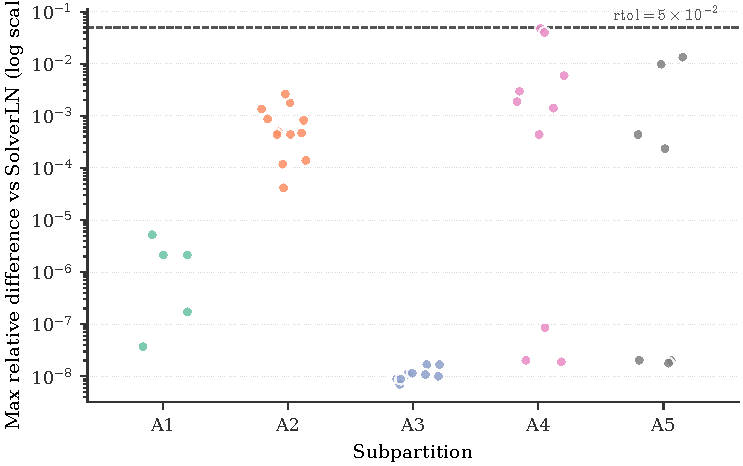
\includegraphics[width=0.68\textwidth]{figures/eval-e31-partition-a-reldiff.pdf}
  \caption[Per-fixture max relative difference on Partition A]{
    Per-fixture maximum relative difference between \texttt{SolverLNSimple}
    and \texttt{SolverLN} on Partition A.
  }
  \label{fig:eval-partition-a-reldiff}
\end{figure}

\textbf{Why the seven Partition~C failures are expected.} All seven \texttt{match-neither} fixtures sit in three of the boundary subpartitions (C5, C6, C7), seen in Table~\ref{tab:eval-correctness-map}. They are constructed specifically to push the simple solver's closed-form kernels past the regimes they are derived for. The three saturated fan-out fixtures (C5) drive per-server utilisation to $\rho \approx 0.99$, where the simple solver's closed-PFQN M/M/c queueing tail and \texttt{SolverLN}'s M/M/$\infty$-like \texttt{R$\approx$D} host substitution diverge. The two AND-fork fixtures (C6) drive the closed-form $E[\max]$ join correction past its independent-server assumption. The two deep all-Exp chain fixtures (C7) converge quickly but to a steady state differing from both references, locating where the bare-demand closed-form kernel transitions under tight coupling.

% C5: --- absorbing them needs a higher-moment or open-system inner kernel, a kernel switch rather than a coupling-layer extension


\section{Iteration-count comparison}
\label{sec:eval-iteration-comparison}

The chapter's headline claim is that \texttt{SolverLNSimple} converges in substantially fewer outer iterations than the two comparator solvers across the corpus. This section reports those counts, inspects them by model partition for clarity, and acknowledges the one comparison bias towards \texttt{SolverLNSimple}'s count (\texttt{SolverLN}'s +2 hard-reset offset). With all three solvers sweeping in an elevator pattern, the counts are otherwise like-for-like.

\subsubsection*{Total iteration counts.} 
Across the 78-fixture corpus, \texttt{SolverLNSimple} uses 539 outer iterations in total, \texttt{SolverLN} uses 4,835 and LQNS uses 985 on the 77 fixtures it can solve. The simple solver runs in 9x fewer iterations than \texttt{SolverLN} (reduced to 8.7x once the +2 offset is removed) and 1.8x fewer than LQNS on the corpus.

\subsubsection*{\texttt{SolverLN}'s \texttt{iter\_min} floor is binding on 63 of 78 fixtures.} 
Of the 78 baseline fixtures, 63 report \texttt{ln\_iters = 53} exactly (the \texttt{iter\_min = 50} floor plus the 2 hard-reset bias and one verification iteration). The fifteen exceptions come from Partition B's large task count chains and fanouts as well as Partition C's saturated fanouts and a deep chain. On these, \texttt{SolverLN}'s convergence is topology-driven, however on the remaining 63, the floor is strictly binding and the iteration-count comparison is simply a comparison of detection rules rather than convergence rates. This motivates the \texttt{iter\_min} ablation study in Section \ref{sec:eval-f20}, investigating the underlying convergence behaviour and allowing the comparison to be more insightful. The per-partition counts behind these totals are reported in Table~\ref{tab:eval-iter-counts-per-partition}.

\begin{table}[h] 
\centering 
\footnotesize
\begin{tabular}{|l|l|l|l|l|l|l|}
\hline
Partition & N & Sim mean & LN mean & LQNS mean & Sim ÷ LN & Sim ÷ LQNS \\
\hline
A1 (single-class chains) & 5 & \textbf{4.4} & 53.0 & 22.0 & \textbf{0.08x} & \textbf{0.20x} \\
\hline
A2 (multi-class shared callee) & 12 & \textbf{3.0} & 53.0 & 9.7 & \textbf{0.06x} & \textbf{0.31x} \\
\hline
A3 (multi-server PS) & 9 & \textbf{4.0} & 53.0 & 7.0 & \textbf{0.08x} & \textbf{0.57x} \\
\hline
A4 (mixed topology) & 10 & \textbf{5.2} & 53.0 & 8.2 & \textbf{0.10x} & \textbf{0.63x} \\
\hline
A5 (activity-graph precedence) & 7 & \textbf{3.6} & 53.0 & 7.5* & \textbf{0.07x} & \textbf{0.48x*} \\
\hline
B (scale axis) & 10 & \textbf{8.3} & 109.8 & 19.9 & \textbf{0.08x} & \textbf{0.42x} \\
\hline
C1 (fan-out callers) & 6 & \textbf{11.0} & 53.0 & 7.3 & \textbf{0.21x} & 1.50x \\
\hline
C2 (INF-task hosts) & 3 & \textbf{3.0} & 53.0 & 2.0 & \textbf{0.06x} & 1.50x \\
\hline
C3 (multi-class × multi-entry) & 3 & \textbf{3.0} & 53.0 & 9.3 & \textbf{0.06x} & \textbf{0.32x} \\
\hline
C4 (boundary cases) & 3 & \textbf{3.7} & 53.0 & 7.7 & \textbf{0.07x} & \textbf{0.48x} \\
\hline
C5 (saturated fan-out) & 6 & \textbf{28.0} & 74.7 & 24.5 & \textbf{0.37x} & 1.14x \\
\hline
C6 (AND-fork join boundary) & 2 & \textbf{3.5} & 53.0 & 29.0 & \textbf{0.07x} & \textbf{0.12x} \\
\hline
C7 (deep chains) & 2 & \textbf{7.5} & 54.5 & 32.0 & \textbf{0.14x} & \textbf{0.23x} \\
\hline
\textbf{TOTAL} & \textbf{78} & \textbf{6.9} & \textbf{62.0} & \textbf{12.8} & \textbf{0.11x} & \textbf{0.54x} \\
\hline
\end{tabular}
{\footnotesize *LQNS unavailable for 1 of 7 A5 fixtures}
\caption{Mean outer-iteration counts per solver per partition.}
\label{tab:eval-iter-counts-per-partition}
\end{table}

\subsubsection*{Per-partition aggregates.}
As mentioned above, on every subpartition of A and most subpartitions of C, \texttt{SolverLN}'s mean iteration count is exactly 53, hitting the \texttt{iter\_min} floor. Partition B varies on the larger task count fixtures designed to test the scalability of the solvers, where genuine topology-driven convergence carries \texttt{SolverLN}'s count above the floor. On this partition, the iteration gap widens further to a 13x ratio. LQNS sits between the two. On raw iteration counts, the simple solver beats LQNS on ten of thirteen partitions, losing on just C1, C2 and C5. On these cases, C2 (2 vs 3) and C5 (just 1.14x) are trivial, but C1 is more informative. The diagnosis is that our fixed \texttt{callerFansOut}-gated $\alpha_Z = 0.5$ damping is on from sweep 1, slowing convergence by design as the price of keeping the saturated fan-out fixtures off the iteration limit (Table~\ref{tab:alpha-tol}). LQNS avoids this with adaptive under-relaxation, only engages once oscillation is detected. This is therefore one case where omission of a more complex mechanism costs iterations rather than saving them, marking the limit of the chapter's wider claim.


\subsubsection*{Per-fixture distribution.}
Figure~\ref{fig:eval-iters-by-solver} visualises each fixture's iteration count across the three solvers, further strengthening the previous findings' claims. The \texttt{SolverLN} points cluster at 53 because of the \texttt{iter\_min} floor on most partitions. The \texttt{SolverLNSimple} points are lowest for the majority of fixtures, while the LQNS counts typically sit between the two.

\begin{figure}[h]
  \centering
  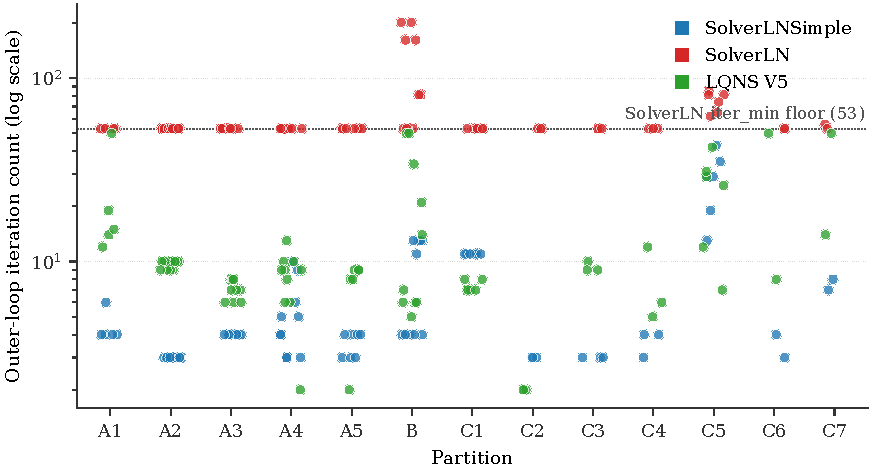
\includegraphics[width=0.8\textwidth]{figures/eval-e41-iters-by-solver.pdf}
  \caption[Outer-loop iteration counts per solver, faceted by partition]{
    Per-fixture outer-loop iteration counts for the three solvers.
  }
  \label{fig:eval-iters-by-solver}
\end{figure}






\section{Runtime comparison}
\label{sec:eval-runtime}

Iteration-count savings translate into wall-clock savings only if per-iteration costs are comparable. This section reports the per-fixture runtime comparison across all three solvers. As iteration counts vary across solvers, we also look into the per-iteration costs. However, again, this shouldn't be an exact comparison due to two asymmetries. Firstly, the LQNS time includes the REST round-trip to the Docker container that hosts LQNS, contributing a measured median 20 ms per call. In the opposite direction however, LQNS is a mature C++ implementation with decades of performance tuning, whereas \texttt{SolverLNSimple} is a Java/Kotlin prototype with limited bespoke runtime optimisation, just the primitive MVA kernels and graph caches.

\subsubsection*{Aggregate wall-clock across the three solvers.}
Across the 78-fixture corpus, \texttt{SolverLN} takes 2,917,118 ms, LQNS takes 23,431 ms (on the 77 fixtures it can solve) and \texttt{SolverLNSimple} takes 22,184 ms. This positions \texttt{SolverLNSimple} 131x faster than \texttt{SolverLN} and 1.06x faster than LQNS as measured, with this reducing to 0.99x once the $\sim$20 ms REST round-trip overhead is subtracted. The large gap to \texttt{SolverLN} sets the size of the runtime discrepancy our per-machinery decomposition later in the chapter characterises. Table~\ref{tab:eval-runtime-per-partition} breaks these totals down by partition and per-fixture mean.

\begin{table}[h]
\centering
\footnotesize
\setlength{\tabcolsep}{4pt}
\begin{tabular}{|>{\raggedright\arraybackslash}p{3.6cm}|l|l|l|l|l|l|l|}
\hline
Partition & N & Sim total & LQNS total & LN total & Sim mean & LQNS mean & LN mean \\
\hline
A1 (single-class chains) & 5 & 116 & 183 & 15,350 & 23 & 37 & 3,070 \\ \hline
A2 (multi-class shared callee) & 12 & 147 & 335 & 13,321 & 12 & 28 & 1,110 \\ \hline
A3 (multi-server PS) & 9 & 65 & 243 & 4,342 & 7 & 27 & 482 \\ \hline
A4 (mixed topology) & 10 & 309 & 282 & 23,952 & 31 & 28 & 2,395 \\ \hline
A5 (activity-graph precedence) & 7 & 1,402 & 234* & 85,303 & 200 & 39* & 12,186 \\ \hline
B (scale axis) & 10 & 18,649 & 20,928 & 2,631,495 & 1,865 & 2,093 & 263,150 \\ \hline
C1 (fan-out callers) & 6 & 103 & 175 & 7,326 & 17 & 29 & 1,221 \\ \hline
C2 (INF-task hosts) & 3 & 27 & 91 & 3,903 & 9 & 30 & 1,301 \\ \hline
C3 (multi-class \texttimes{} multi-entry) & 3 & 39 & 83 & 3,215 & 13 & 28 & 1,072 \\ \hline
C4 (boundary cases) & 3 & 19 & 79 & 1,531 & 6 & 26 & 510 \\ \hline
C5 (saturated fan-out) & 6 & 638 & 663 & 78,978 & 106 & 110 & 13,163 \\ \hline
C6 (AND-fork join boundary) & 2 & 633 & 76 & 44,929 & 316 & 38 & 22,464 \\ \hline
C7 (deep chains) & 2 & 37 & 59 & 3,473 & 18 & 30 & 1,736 \\ \hline
\textbf{TOTAL} & \textbf{78} & \textbf{22,184} & \textbf{23,431} & \textbf{2,917,118} & \textbf{284} & \textbf{304} & \textbf{37,399} \\
\hline
\end{tabular}
{\footnotesize LQNS unavailable for 1 of 7 A5 fixtures.}
\caption{Per-partition wall-clock totals and per-fixture means, all values in milliseconds.}
\label{tab:eval-runtime-per-partition}
\end{table}

\subsubsection*{Per-partition wall-clock concentrates on Partition B.}
Partition B alone is 90.2\% of \texttt{SolverLN}'s, 89.3\% of LQNS's and 84.1\% of \texttt{SolverLNSimple}'s corpus total, identifying the partition's per-layer MVA solve as its cost bottleneck. The $\sim$20 ms LQNS floor visible in the eleven non-B/C6 partitions is the REST round-trip overhead mentioned. Focusing on partition B gives us a cleaner comparison of the solvers' per-iteration cost as REST calls, JIT state, and other sources of noise impact is minimised. When comparing partition B runtimes, we see \texttt{SolverLNSimple} as 1.12x faster than LQNS. Figure~\ref{fig:eval-runtime-by-solver} plots the per-fixture runtimes across all three solvers.

\begin{figure}[h]
  \centering
  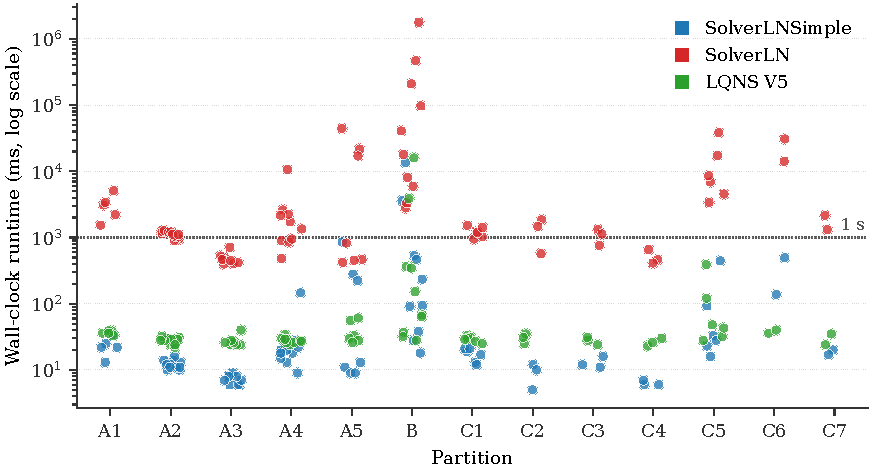
\includegraphics[width=0.8\textwidth]{figures/eval-e52-fair-runtime-by-solver.pdf}
  \caption[Per-fixture wall-clock runtime per solver, fair-bracket Sim, medianed]{
    Per-fixture wall-clock runtime for the three solvers.
  }
  \label{fig:eval-runtime-by-solver}
\end{figure}

\subsubsection*{Per-iteration runtime on Partition B across all three solvers.} 
Because iteration counts vary across solvers, the load-bearing comparison is per-iteration rather than aggregate (Table~\ref{tab:eval-per-iter-runtime-baseline}). LQNS wins on the five chain fixtures and \texttt{SolverLNSimple} wins on the five fanouts.

\begin{table}[h]
\centering
\footnotesize
\setlength{\tabcolsep}{3pt}
\resizebox{\linewidth}{!}{%
\begin{tabular}{|l|r|r|r|r|r|r|r|r|}
\hline
Fixture & LN it & LN ms/it § & LQNS it & LQNS ms/it & Sim it & Sim ms/it & LN/Sim & LQNS/Sim \\
\hline
\texttt{B\_scaleAxis\_tasks5\_chain} & 53 & 52.81 & 14 & \textbf{2.00} & 4 & 4.50 & 11.7x & 0.44x \\ \hline
\texttt{B\_scaleAxis\_tasks5\_fanout} & 53 & 63.02 & 6 & 5.33 & 13 & \textbf{2.15} & 29.3x & 2.48x \\ \hline
\texttt{B\_scaleAxis\_tasks10\_chain} & 53 & 112.5 & 21 & \textbf{1.76} & 4 & 9.50 & 11.8x & 0.19x \\ \hline
\texttt{B\_scaleAxis\_tasks10\_fanout} & 53 & 152.6 & 7 & 9.71 & 13 & \textbf{7.00} & 21.8x & 1.39x \\ \hline
\texttt{B\_scaleAxis\_tasks20\_chain} & 81 & 222.2 & 34 & \textbf{1.88} & 4 & 23.50 & 9.5x & 0.08x \\ \hline
\texttt{B\_scaleAxis\_tasks20\_fanout} & 81 & 503.6 & 6 & 60.50 & 13 & \textbf{41.00} & 12.3x & 1.48x \\ \hline
\texttt{B\_scaleAxis\_tasks40\_chain} & 161 & 604.9 & 50 & \textbf{3.04} & 4 & 58.75 & 10.3x & 0.05x \\ \hline
\texttt{B\_scaleAxis\_tasks40\_fanout} & 161 & 2,916.7 & 6 & 645.0 & 13 & \textbf{277.6} & 10.5x & 2.32x \\ \hline
\texttt{B\_scaleAxis\_tasks60\_chain} & 201 & 1,041.5 & 50 & \textbf{6.92} & 4 & 117.5 & 8.9x & 0.06x \\ \hline
\texttt{B\_scaleAxis\_tasks60\_fanout} & 201 & 8,836.8 & 5 & 3,193.6 & 11 & \textbf{1,230.3} & 7.2x & 2.60x \\ \hline
\end{tabular}%
}
\caption{Per-iteration wall-clock on Partition B.}
\label{tab:eval-per-iter-runtime-baseline}
\end{table}

The \texttt{SolverLN}/\texttt{SolverLNSimple} ratio shows \texttt{SolverLNSimple} 7.2-29.3x cheaper per iteration than \texttt{SolverLN} on every Partition B fixture. Combined with the previous section's iteration-count savings, this is the first evidence that suggests \texttt{SolverLNSimple}'s lead over \texttt{SolverLN} extends beyond convergence detection and into raw per-iteration cost, and the gap reflects genuine algorithmic machinery. 

The LQNS/\texttt{SolverLNSimple} ratio inverts across the two shapes, 0.05x--0.44x for chains and 1.39x--2.60x for fan-outs, reflecting a difference in decomposition. \texttt{SolverLNSimple} splits the model one layer per task and processor, so every callee is a single-class submodel, width never enters any MVA's class count, paying for depth in per-sweep work and for width in iteration count. LQNS keeps narrow-deep chain submodels cheap by paying for depth in iterations instead, but its per-iteration solve grows steeply with fan-out width.

\subsubsection*{\texttt{SolverLNSimple}'s activity graph runtime gap is not a per-iteration solve cost.} 
Partition A5 loses to LQNS on wall-clock greatly (200 ms mean vs 39 ms). However, of A5's 1,402 ms \texttt{SolverLNSimple} total, 1,260 ms of it is accounted for by the three AND-fork fixtures, despite all converging in three iterations, and the other A5 fixtures converging in 2--3 ms. The partition-level ``activity graphs are slow'' reading is therefore false, and the cost is specific to the AND-fork→AND-join construct. Table~\ref{tab:eval-a5-construct-split} separates construction from iteration cost for representative A5 fixtures.

\begin{table}[h]
\centering
\footnotesize
\setlength{\tabcolsep}{4pt}
\begin{tabular}{|l|r|r|r|}
\hline
A5 fixture & \texttt{getEnsemble} ms & \texttt{iterate} ms & LQNS ms \\
\hline
\texttt{combinedDag}     & 894 & 4.4 & --- \\ \hline
\texttt{andForkMultiAct} & 276 & 3.7 & 33 \\ \hline
\texttt{andForkThreeWay} & 225 & 3.5 & 30 \\ \hline
\texttt{orForkThreeWay}  &  18 & 5.0 & 56 \\ \hline
\texttt{orForkUneven}    &  19 & 5.6 & 61 \\ \hline
\end{tabular}
\caption{Construction versus iteration wall-clock for representative A5 fixtures (separate instrumented profiling, warm JVM, $N=100$). The fixed-point solve is flat; the AND-fork penalty is entirely in \texttt{getEnsemble}.}
\label{tab:eval-a5-construct-split}
\end{table}

A profiling run shows the coupled-MVA fixed point is flat at 3.5--5.6 ms for \textit{every} A5 fixture, and the entire delay is in construction, rising from $\sim$18 ms on the OR-fork fixtures to 225-894 ms on the AND-fork fixtures. We can therefore determine that the iterative solver itself, including the $E[\max]$ join-delay machinery of the AND-fork throughput correction, is cheap, and it is instead the ensemble construction, that we have inherited from \texttt{SolverLN} that is expensive.

We see that construction calls \texttt{getStruct} on each per-task submodel, whose cost is dominated by the visit-ratio linear solves (\texttt{dtmc\_solve}, \texttt{Matrix.solveSafe}). Fork/join branches give a richer routing matrix than other paradigms, so this generic refresh scales. LQNS, a native LQN solver, never builds a flat queueing network per task, so construction time stays low. We therefore get penalised for using \texttt{SolverLN}'s generic ensemble construction machinery.

\subsubsection*{LQNS net of REST round-trip overhead.}
We instrument \texttt{SolverLQNS} to record per-call \texttt{rest\_call\_ms} (the HTTP block enclosing the remote solve) and \texttt{lqns\_elapsed\_ms} (the kernel solve, parsed from the LQXO). Their difference gives a median REST round-trip overhead of 20 ms per call. Subtracting this from each of the 77 solvable LQNS results, the LQNS corpus total drops from 23,431 ms to 21,891 ms, tightening \texttt{SolverLNSimple} ÷ LQNS from 1.06x to 0.99x. We see that whilst most partitions lose their floor and drop below \texttt{SolverLNSimple}, partition B and C5 stay relatively unchanged as they are dominated by kernel time. Figure~\ref{fig:eval-runtime-by-solver-no-rest} re-plots the per-fixture runtimes with this overhead removed from the LQNS results.

\begin{figure}[h]
  \centering
  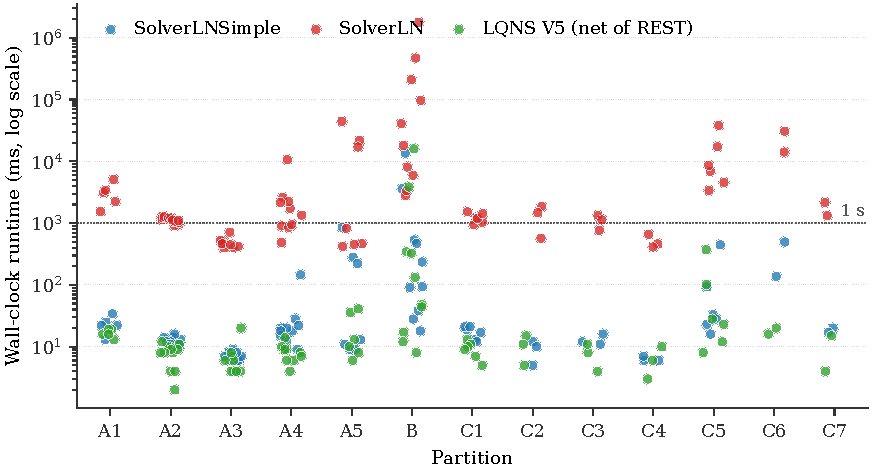
\includegraphics[width=0.8\textwidth]{figures/eval-e52b-lqns-no-rest.pdf}
  \caption[Per-fixture runtime, LQNS net of REST overhead]{
    Figure~\ref{fig:eval-runtime-by-solver} with LQNS V5 (green) net of REST overhead. Sim and LN unchanged.
  }
  \label{fig:eval-runtime-by-solver-no-rest}
\end{figure}
 











\section{SolverLN ablations}
\label{sec:eval-ablations}

We hypothesise that the runtime and iteration-count gaps of the previous two sections are produced by specific \texttt{SolverLN} machinery that \texttt{SolverLNSimple} omits. We isolate the two largest contributors by disabling each inside \texttt{SolverLN} and re-measuring against the baseline. \emph{Interlock correction} is a pure runtime-surface cost on this corpus, not affecting iteration count or output, but adding per-iteration work that grows with fan-out breadth. \emph{Convergence control} dominates the iteration-count gap, but carries a small accuracy benefit.

\subsection{Interlock correction}
\label{sec:eval-interlock}

\texttt{SolverLN} runs an LQNS-style interlock subsystem that corrects residence and call-service times when two or more client tasks contend for a shared server task. It does a random walk over the call graph (matrix powers \texttt{P\textasciicircum step}) that estimates the probability each task is transitively called by another, and the correction pipeline that consumes these estimates. On this corpus, neither piece of machinery affects the result as the correction only fires when a server has two or more distinct client tasks, yet this is not a topology we have considered. This causes the consumer to short-circuit before computing any adjustment, however the random walk's output (\texttt{ptaskcallers}) has already been computed. The subsystem is therefore predicted to add per-iteration cost with no iteration-count and no accuracy effect.

\subsubsection*{Zero iteration-count and zero accuracy effect.} 
Disabling the whole subsystem leaves every fixture's iteration count identical to baseline (corpus total 4,835) and every output metric unchanged. This is not a claim that interlock is useless in general, but that on a corpus that never triggers it, the machinery runs every iteration and pays its full per-iteration cost for no benefit.

\subsubsection*{Per-iteration cost grows with fan-out breadth.} 
The cost removed from disabling interlock correction grows along two axes (Table~\ref{tab:eval-interlock-per-iter}). On chains, we see that it rises modestly with depth (1.37$\times$--1.46$\times$), tracking the random walk's matrix-power cost as the call graph grows. On fan-outs it rises far more steeply with width (1.0$\times$--2.77$\times$). The steeper increase is caused by the correction pipeline's per-iteration data-structure refresh, where the fan-out caller's host layer carries one closed class per outgoing synchronous call. The cut closes the widest fan-out's  per-iteration gap to \texttt{SolverLNSimple} down from 7.2$\times$ to just 2.6$\times$ (raw runtime decreases from 8,836 ms to 3,186 ms). Figure~\ref{fig:eval-interlock-speedup} plots this per-iteration speedup by task count and topology.

\begin{table}[h]
\centering
\footnotesize
\setlength{\tabcolsep}{4pt}
\begin{tabular}{|l|r|r|r|r|r|r|}
\hline
Fixture & LN iters & base ms/it & intlk-off ms/it & speedup & Sim ms/it & intlk-off/Sim \\
\hline
\texttt{B\_scaleAxis\_tasks5\_chain}   & 53  & 52.8    & 52.4    & 1.01x & 4.5     & 11.6x \\ \hline
\texttt{B\_scaleAxis\_tasks10\_chain}  & 53  & 112.5   & 96.9    & 1.16x & 9.5     & 10.2x \\ \hline
\texttt{B\_scaleAxis\_tasks20\_chain}  & 81  & 222.2   & 235.8   & 0.94x & 23.5    & 10.0x \\ \hline
\texttt{B\_scaleAxis\_tasks40\_chain}  & 161 & 604.9   & 439.9   & 1.37x & 58.8    & 7.5x  \\ \hline
\texttt{B\_scaleAxis\_tasks60\_chain}  & 201 & 1,041.5 & 712.7   & 1.46x & 117.5   & 6.1x  \\ \hline
\texttt{B\_scaleAxis\_tasks5\_fanout}  & 53  & 63.0    & 71.3    & 0.88x & 2.2     & 33.1x \\ \hline
\texttt{B\_scaleAxis\_tasks10\_fanout} & 53  & 152.6   & 167.2   & 0.91x & 7.0     & 23.9x \\ \hline
\texttt{B\_scaleAxis\_tasks20\_fanout} & 81  & 503.6   & 382.1   & 1.32x & 41.0    & 9.3x  \\ \hline
\texttt{B\_scaleAxis\_tasks40\_fanout} & 161 & 2,916.7 & 1,283.2 & \textbf{2.27x} & 277.6   & 4.6x  \\ \hline
\texttt{B\_scaleAxis\_tasks60\_fanout} & 201 & 8,836.8 & 3,186.0 & \textbf{2.77x} & 1,230.3 & \textbf{2.6x} \\ \hline
\end{tabular}
\caption{Per-iteration cost on Partition B, comparing the baseline with the interlock subsystem disabled.}
\label{tab:eval-interlock-per-iter}
\label{tab:eval-f24-per-partition}
\end{table}

\begin{figure}[h]
  \centering
  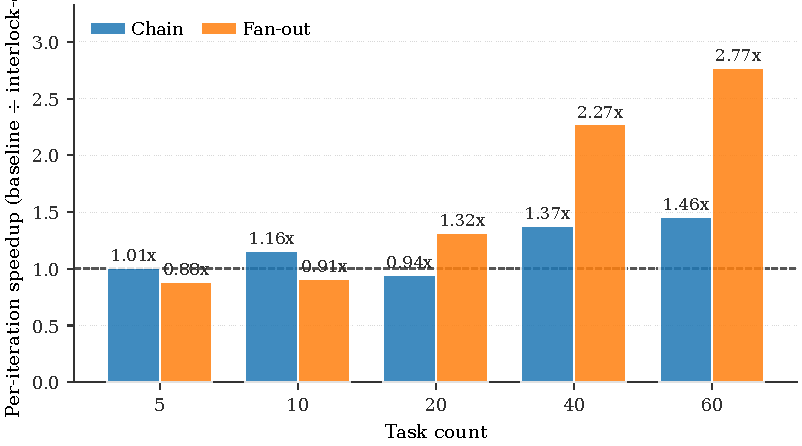
\includegraphics[width=0.8\textwidth]{figures/eval-e61-interlock-speedup-partitionb.pdf}
  \caption[Interlock-off per-iteration speedup on Partition B]{
    Per-iteration speedup from disabling the interlock subsystem on Partition B, by task count and topology.
  }
  \label{fig:eval-interlock-speedup}
\end{figure}

\textbf{Accuracy on interlock-triggering topologies.} The zero-accuracy result above is scoped to the corpus, which never fires the correction. To check whether the correction matters where it is supposed to fire, we ran a small separate probe of four diamond-shaped fixtures in which a reference task fans out to two intermediates that call a shared single-server FCFS server, breaking the independence assumption. Each fixture is solved with the interlock correction on and off and compared against an \texttt{lqsim} ground truth with 100k samples (Table~\ref{tab:eval-interlock-accuracy-probe}). The contribution is the change in worst-case relative difference vs \texttt{lqsim} across \{QLen, RespT, Tput\}. On every fixture, interlock-on is closer to \texttt{lqsim} than interlock-off by $+0.19$ to $+1.41$ percentage points. The contribution is small but directionally consistent. On the multiclass fixture, it also moved the iteration count down from 68 to 53. The corpus-aggregate ``zero accuracy effect'' is therefore scope-bound rather than a no-op claim about the machinery: interlock is genuine accuracy machinery on topologies that trigger it, and this corpus simply never does.

\begin{table}[h]
\centering
\footnotesize
\begin{tabular}{|l|r|r|r|r|r|}
\hline
Fixture & intlk-on & intlk-off & $\Delta$ (contrib) & on iters & off iters \\
\hline
\texttt{directInterlock\_n8}     & 3.23\% & 3.96\% & $+0.73$\,pp & 53 & 53 \\ \hline
\texttt{directInterlock\_n16}    & 0.86\% & 1.05\% & $+0.19$\,pp & 53 & 53 \\ \hline
\texttt{transitiveInterlock\_n8} & 2.98\% & 3.26\% & $+0.28$\,pp & 83 & 83 \\ \hline
\texttt{multiclassInterlock}     & 4.86\% & 6.27\% & $+1.41$\,pp & 53 & 68 \\ \hline
\end{tabular}
\caption{Worst-case relative difference vs the \texttt{lqsim} ground truth on small diamond-shaped fixtures that trigger the interlock correction.}
\label{tab:eval-interlock-accuracy-probe}
\end{table}

Two limitations we came across were a bug in SolverLN, where both interlock-on and interlock-off showed a $\sim$50\% error for some fixtures. We are also only able test accuracy on small fixtures as otherwise it would become too costly to run the \texttt{lqsim} ground truth. However, this means we do not know if the correction's contribution grows with scale.



\subsection{Convergence control}
\label{sec:eval-f20}
\label{sec:eval-iter-min}

\texttt{SolverLN.converged(it)} decides when the fixed-point iteration may stop. It bundles four pieces of machinery: an \texttt{iter\_min} floor (= \texttt{max(2$\cdot$E, ceil(iter\_max/4))}) that delays convergence until a minimum iteration count, a sliding-window weighted average over \texttt{Q}/\texttt{U}/\texttt{R}/\texttt{T} that smooths per-iteration metric noise, a three-iteration confirmation and a hard-reset verification pass. \texttt{SolverLNSimple} replaces the entirety with a single-iteration test, stopping the moment the per-layer throughput delta falls below \texttt{iter\_tol}. This is the single largest contributor to the iteration-count gap. Disabling it, again, carries a small accuracy cost.

\subsubsection*{Disabling complex convergence logic cuts iteration count by 65\%.} 
The corpus total drops from 4,835 to 1,672 outer iterations (2.89$\times$). The reduction concentrates on the floor, as 65 of the 78 fixtures sit at exactly 53 iterations but now collapse to single digits, exposing their true convergence point. The thirteen exceptions are Partition B's large chains and fan-outs and Partition C's saturated fan-outs and deep chains, where convergence is genuinely topology-driven above the floor, where the gap closes by $\sim$50\% rather than $\sim$80\%. However even at 1,672, \texttt{SolverLN} still sits 3.1$\times$ above \texttt{SolverLNSimple}'s 539, so the convergence machinery accounts for most but not all of the gap. Table~\ref{tab:eval-f20-iter-counts} gives the per-partition breakdown and the resulting gap closure.

\begin{table}[h]
\centering
\small
\begin{tabular}{|l|l|l|l|l|l|l|}
\hline
Partition & N & Sim & Baseline LN & Conv-off LN & Reduction & Gap closure \\
\hline
A1 & 5 & 22 & 265 & 74 & 3.58x & 78.6\% \\ \hline
A2 & 12 & 36 & 636 & 194 & 3.28x & 73.7\% \\ \hline
A3 & 9 & 36 & 477 & 108 & 4.42x & 83.7\% \\ \hline
A4 & 10 & 52 & 530 & 135 & 3.93x & 82.6\% \\ \hline
A5 & 7 & 25 & 371 & 70 & 5.30x & 87.0\% \\ \hline
B & 10 & 83 & 1,098 & 521 & 2.11x & 56.8\% \\ \hline
C1 & 6 & 66 & 318 & 96 & 3.31x & 88.1\% \\ \hline
C2 & 3 & 9 & 159 & 30 & 5.30x & 86.0\% \\ \hline
C3 & 3 & 9 & 159 & 40 & 3.98x & 79.3\% \\ \hline
C4 & 3 & 11 & 159 & 32 & 4.97x & 85.8\% \\ \hline
C5 & 6 & 168 & 448 & 309 & 1.45x & 49.6\% \\ \hline
C6 & 2 & 7 & 106 & 16 & 6.62x & 90.9\% \\ \hline
C7 & 2 & 15 & 109 & 47 & 2.32x & 66.0\% \\ \hline
\textbf{TOTAL} & \textbf{78} & \textbf{539} & \textbf{4,835} & \textbf{1,672} & \textbf{2.89x} & \textbf{73.6\%} \\ \hline
\end{tabular}
\caption{Per-partition outer-iteration counts with the convergence control disabled, and the resulting closure.}
\label{tab:eval-f20-iter-counts}
\label{tab:eval-gap-closure}
\end{table}

\subsubsection*{A small accuracy cost.} 
The smoothing arms are what \texttt{SolverLNSimple} gives up for speed. Measuring \texttt{SolverLN}'s own per-cell output with and without the convergence machinery, we see that 7 of the 78 fixtures drift by more than 5\% on some cell, ranging up to 32\% (Table~\ref{tab:eval-f20-accuracy-losses}). The drift concentrates on cells that oscillate around the fixed point (per-class shared-callee queue lengths, low-demand response times, asymmetric multi-entry residence times). These are cells where the moving average smoothing would usually have an effect. \texttt{SolverLN}'s convergence detection takes the windowed-maximum error rather than the current-iteration error. Without it, detection can fire on a one-off low during an oscillation phase, with the response characterising whatever phase the iteration was in. The accuracy cost is from the moving-average smoothing and hard-reset arm, as the \texttt{iter\_min} floor just delays convergence to the same fixed point. The correctness results (Section~\ref{sec:eval-correctness}) show \texttt{SolverLNSimple} still lands within tolerance of a reference on these fixtures, so the omission is acceptable on this corpus, but we do recognise the small accuracy cost. It is also unfair to take these drifts at face value, as \texttt{SolverLN} was not built with a run like this in mind.

\begin{table}[h]
\centering
\footnotesize
\setlength{\tabcolsep}{5pt}
\resizebox{\linewidth}{!}{%
\begin{tabular}{|l|l|r|l|l|}
\hline
Fixture & Part. & Drift & Worst cell (base $\to$ conv-off) & Mechanism \\
\hline
\texttt{A2\_multiclassA\_2refs\_loadHigh\_N50} & A2 & 32.0\% & \texttt{R2.qlen} (49.3 $\to$ 65.1) & per-class shared-callee oscillation \\ \hline
\texttt{C4\_lowDemand} & C4 & 28.2\% & \texttt{E1.respt} (0.052 $\to$ 0.067) & low-load tolerance-boundary oscillation \\ \hline
\texttt{C3\_multiclassMultiEntry\_asymmetric} & C3 & 15.8\% & \texttt{AS1.residt} (1.58 $\to$ 1.83) & asymmetric multi-entry shared callee \\ \hline
\texttt{A2\_multiclassA\_2refs\_loadHigh\_N20} & A2 & 12.6\% & \texttt{R2.qlen} (19.3 $\to$ 21.8) & per-class shared-callee oscillation \\ \hline
\texttt{A2\_multiclassA\_2refs\_loadLow\_N50} & A2 & 12.3\% & \texttt{R1.qlen} (48.0 $\to$ 53.9) & per-class shared-callee oscillation \\ \hline
\texttt{C5\_satFanoutCaller\_w2} & C5 & 7.4\% & \texttt{TS1.qlen} (3.78 $\to$ 4.06) & saturated fan-out caller oscillation \\ \hline
\texttt{C7\_deepChainMultiCall} & C7 & 6.4\% & \texttt{T2.residt} (0.30 $\to$ 0.32) & deep multi-call chain oscillation \\ \hline
\end{tabular}%
}
\caption{The seven fixtures whose \texttt{SolverLN} output drifts by more than 5\% when the convergence control is disabled.}
\label{tab:eval-f20-accuracy-losses}
\end{table}

\subsection{The residual algorithmic difference}
\label{sec:eval-residual}

The convergence machinery does not explain the whole gap in runtime and iteration count as with it disabled, \texttt{SolverLN} still uses 1,672 iterations against \texttt{SolverLNSimple}'s 539. The cut therefore closes $(4{,}835-1{,}672)/(4{,}835-539) = 73.6\%$ of the iteration-count gap, where the remaining $\approx$26\% (1,133 iterations corpus-wide) is genuine algorithmic difference between the two solvers, not just convergence machinery. Per partition, the closure ranges from $\approx$50\% on Partition B and C5, where \texttt{SolverLN}'s convergence is genuinely slower than the simple solver's, to $\approx$90\% on C6 (Figure~\ref{fig:eval-gap-closure}). The residual comes from the simple solver's three structural choices that the contribution chapter names: predicate-gated $\alpha_Z$ damping fired only where it is needed rather than \texttt{SolverLN}'s unconditional blend, structural service-time propagation rather than \texttt{*\_prev} snap-back arrays to handle failures, and single-iteration convergence detection providing looser guarantees rather than three-iteration confirmation.

\begin{figure}[h]
  \centering
  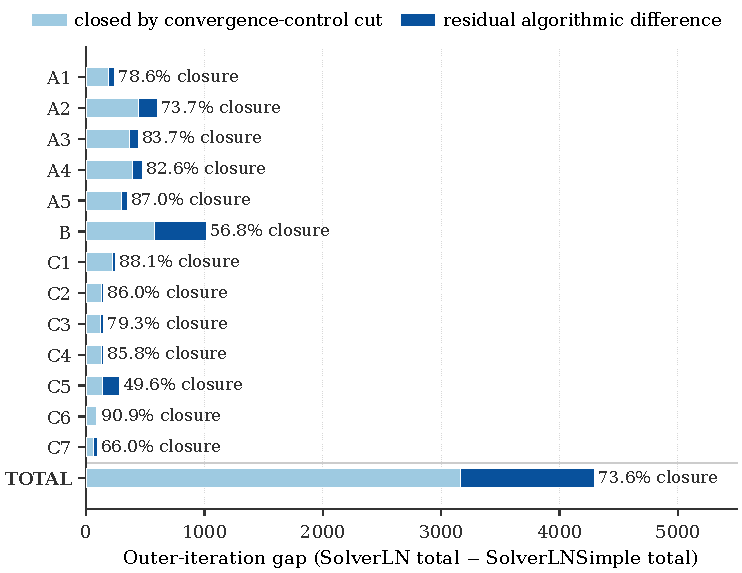
\includegraphics[width=0.72\textwidth]{figures/eval-e91-gap-closure-decomposition.pdf}
  \caption[Per-partition iteration-count gap closure]{
    Decomposition of the \texttt{SolverLN}-vs-\texttt{SolverLNSimple} iteration-count gap per partition. Each bar's total length is the per-partition gap (\texttt{baseline LN} $-$ \texttt{Sim}), split into a light portion closed by disabling the convergence control and a dark residual algorithmic difference. The aggregate split is 73.6\% / 26.4\%; per-partition closure ranges from $\approx$50\% (B, C5) to $\approx$90\% (C6).
  }
  \label{fig:eval-gap-closure}
\end{figure}






\section{The accuracy boundary} 
\label{sec:eval-boundary}
\label{sec:eval-failure-modes}

This section maps where the \texttt{SolverLNSimple} and \texttt{SolverLN} diverge. Of the 78 fixtures the 57 \texttt{match-ln} are graded in Section~\ref{sec:eval-correctness} and the other 21 are characterised here. Fourteen are divergent-by-design, where they match LQNS instead when the reference solvers diverge. Seven match neither reference, whose structural causes were previously named in correctness Section~\ref{sec:eval-correctness}. Therefore every divergence is accounted for and none disagree with our correctness claims.

\textbf{A host-layer modelling divergence that matches LQNS.} The fourteen \texttt{match-lqns-only} fixtures (six C1 fan-out callers, five B fan-out fixtures, three C5 saturated fan-outs) sit 28\%--81\% from \texttt{SolverLN} but $\leq$7.7e-02 from LQNS (Table~\ref{tab:eval-divergent-partitions-reldiff}). The cause is a difference in host-layer modelling where at moderate-to-high per-server utilisation \texttt{SolverLN} collapses the host residence to its cheap M/M/$\infty$-like \texttt{R$\approx$D} approximation, dropping the queueing term, while \texttt{SolverLNSimple} keeps the closed-PFQN M/M/c queueing tail. The gap widens with fan-out width and grows monotonically with task count, while C1 additionally fires the \texttt{LqnGraph.callerFansOut}-gated fixed-$\alpha$ damping. Whether keeping the queueing tail is more accurate or spurious in trees sized for M/M/$\infty$ behaviour can only be settled by discrete-event simulation (\texttt{lqsim}), which the chapter does not do. The narrower, sound claim is that \texttt{SolverLNSimple} reproduces the established tool's host-layer choice where \texttt{SolverLN} departs from it. This is an interesting case however, as it is \texttt{SolverLNSimple} that opts for more machinery and rigorous computation.

\begin{table}[h]
\centering 
\small
\begin{tabularx}{\linewidth}{|l|l|l|X|}
\hline
Fixture & Partition & sim vs LN max rel diff & Mechanism \\
\hline
\texttt{C1\_fanOut2\_caller\_c1} & C1 & 0.294 & \multirow{6}{=}{Fan-out caller; predicate-gated ($\alpha$) damping disagreement, widening with fan-out width} \\
\cline{1-3}
\texttt{C1\_fanOut2\_caller\_c2} & C1 & 0.294 & \\
\cline{1-3}
\texttt{C1\_fanOut3\_caller\_c1} & C1 & 0.362 & \\
\cline{1-3}
\texttt{C1\_fanOut3\_caller\_c2} & C1 & 0.362 & \\
\cline{1-3}
\texttt{C1\_fanOut4\_caller\_c1} & C1 & 0.303 & \\
\cline{1-3}
\texttt{C1\_fanOut4\_caller\_c2} & C1 & 0.303 & \\
\hline
\texttt{B\_scaleAxis\_tasks5\_fanout}  & B & 0.281 & \multirow{5}{=}{M/M/$\infty$-vs-M/M/c host approximation at moderate $\rho$; grows monotonically with task count} \\
\cline{1-3}
\texttt{B\_scaleAxis\_tasks10\_fanout} & B & 0.466 & \\
\cline{1-3}
\texttt{B\_scaleAxis\_tasks20\_fanout} & B & 0.594 & \\
\cline{1-3}
\texttt{B\_scaleAxis\_tasks40\_fanout} & B & 0.723 & \\
\cline{1-3}
\texttt{B\_scaleAxis\_tasks60\_fanout} & B & 0.808 & \\
\hline
\texttt{C5\_satFanout\_tasks5}  & C5 & 0.441 & \multirow{3}{=}{Same M/M/$\infty$-vs-M/M/c boundary, saturated ($\rho \approx 0.99$)} \\
\cline{1-3}
\texttt{C5\_satFanout\_tasks10} & C5 & 0.468 & \\
\cline{1-3}
\texttt{C5\_satFanout\_tasks20} & C5 & 0.605 & \\
\hline
\end{tabularx}
\caption{Maximum relative differences against \texttt{SolverLN} on the match-lqns-only fixtures.}
\label{tab:eval-divergent-partitions-reldiff}
\end{table}

\textbf{The seven \texttt{match-neither} failures.} The Correctness Section~\ref{sec:eval-correctness} named the structural cause of each true failure. The three C5 \textbf{saturated fan-out callers} ($\rho \approx 0.99$) put all three solvers in disagreement (\texttt{sim\_vs\_ln} 0.44--0.55, \texttt{sim\_vs\_lqns} 0.12--0.16), where the M/M/c-vs-M/M/$\infty$ boundary pushed past where any solver is ground truth. We actually require a higher-moment or open-system inner kernel rather than a simple coupling-layer extension. The two C6 \textbf{AND-fork fixtures} break the closed-form $E[\max]$ join correction's independent-server assumption (\texttt{LqnGraph.andForkMaxCorrection}, Heidelberger--Trivedi \cite{heidelberger83}) from opposite sides (via a finite-server PS host and via interacting per-class corrections on a shared callee). These fixtures would require Franks's CCD overlap compensation. The two C7 \textbf{deep all-Exp chains} converge in 3--4 iterations to a steady state differing from both references, locating where the bare-demand kernel transitions under tight coupling.

\textbf{Largest core residual: \texttt{A4\_chainPlusFanout}.} The four-tier multi-class chain with a multi-entry middle tier is \texttt{match-ln} at \texttt{sim\_vs\_ln} = 4.76e-02, just under the \texttt{rtol = 5e-2} bar, converging in 6 outer iterations. It marks multi-class $\times$ multi-entry as the corpus's most accuracy-sensitive subpartition.

\textbf{Out-of-corpus implementation gap: \texttt{minimal\_multiEntryCaller}.} A failing fixture we found that did not make it into the test corpus was the case where a REF caller issues two synchronous calls per cycle to two entries of an intermediate task. Our function to scale leaf-task throughputs skips any task with downstream callees, keeping a per-cycle rather than per-call rate. The coupling is correct, this is only a reporting issue. Extending the scaling pass to intermediates with inbound \texttt{callMean > 1} would fix it.







\section{Findings}
\label{sec:eval-discussion}

This section reads the chapter's measurements against the seven hypotheses, names what the residual algorithmic difference is, separates the genuine reference disagreement from the true failures, and states explicitly what the chapter does and does not claim.

\subsection{Findings against the hypotheses}

\textbf{H1 (correctness): confirmed.} 71 of 78 fixtures pass, and every one of the seven \texttt{match-neither} failures falls in a boundary subpartition (three C5, two C6, two C7). None lands in a positive-evidence partition (Table~\ref{tab:eval-correctness-map}). 

\textbf{H2 (iteration-count reduction): confirmed.} \texttt{SolverLNSimple} uses 539 outer iterations against \texttt{SolverLN}'s 4,835 (9x) and LQNS's 985 (1.8x), and beats \texttt{SolverLN} on every fixture. The only partitions where it loses to LQNS on are C1, C2, and C5, which are either trivial or as a result of fixed-vs-adaptive damping (Section~\ref{sec:eval-iteration-comparison}).

\textbf{H3 (runtime): confirmed.} 22,184 ms against \texttt{SolverLN}'s 2,917,118 ms (131x) and LQNS's 23,431 ms (1.06x faster as measured but 0.99x once the REST round-trip is removed, still a good win for a Java-vs-C++ comparison) (Section~\ref{sec:eval-runtime}).

\textbf{H4 (interlock is a runtime-surface cost): confirmed.} Disabling the correction leaves every fixture's iteration count and output metric unchanged while removing per-iteration cost that grows up to 2.77x on the widest fanout case (Table~\ref{tab:eval-interlock-per-iter}). On a corpus that never triggers the correction, it is a pure per-iteration cost. On models that do trigger it, we see a small accuracy difference (Section~\ref{sec:eval-interlock}).

\textbf{H5 (convergence control dominates the iteration-count gap): confirmed.} Disabling it cuts the corpus from 4,835 to 1,672 iterations (2.89x), closing 73.6\% of the gap. The reduction concentrates on the floor, where most of the fixtures pinned at 53 iterations collapse to single digits, exposing their true convergence point (Section~\ref{sec:eval-f20}).

\textbf{H6 (convergence control accuracy cost): confirmed and quantified.} Seven of 78 fixtures drift by more than 5\% when the smoothing is removed, up to 32\%, all on cells that oscillate around the fixed point (Table~\ref{tab:eval-f20-accuracy-losses}). The cost is real, but mostly concentrated and small (Section~\ref{sec:eval-f20}).

\textbf{H7 (residual remains): confirmed at 26.4\%.} With convergence control off, \texttt{SolverLN} still uses 1,672 iterations against the \texttt{SolverLNSimple}'s 539, a residual the convergence machinery does not explain, which Section~\ref{sec:eval-residual} attributes structurally to the simple solver's coupling and damping choices.




\subsection{What the chapter does not claim}
\label{sec:eval-notclaim}

The chapter does not claim \texttt{SolverLN}'s machinery is redundant in general. The interlock correction is unexercised here only because no corpus fixture instantiates a shared server with two or more distinct client tasks. The diamond probe (Table~\ref{tab:eval-interlock-accuracy-probe}) shows it does real accuracy work where it fires. The convergence smoothing carries a measurable accuracy cost when removed (Table~\ref{tab:eval-f20-accuracy-losses}), so it too is doing useful work on oscillation-prone fixtures. The claim is the narrower one. On this corpus, omitting these machineries recovers most of the iteration-count difference and a large share of the per-iteration runtime at a small, bounded, quantified accuracy cost.

We also don't try to claim correctness in the saturated and AND-fork regimes the seven \texttt{match-neither} fixtures occupy. The three C5 saturated fan-outs ($\rho \approx 0.99$) and two C6 AND-fork fixtures push the simple solver's closed-form kernels past the regimes they are derived for, and the two C7 deep all-Exp chains converge to a steady state differing from both references (Section~\ref{sec:eval-boundary}). These are deliberately adversarial cases outside the claimed scope, surfaced rather than hidden. The boundary section names the concrete extension each failure would need.

Finally, the chapter does not take reference solver outputs at face value. It uses them as a guideline for structural comparison and correctness rather than as ground truth, so the host-layer disagreement it surfaces is characterised, not adjudicated.

Three of these gaps are also the natural next steps. The 26.4\% residual is attributed structurally rather than measured, so ablating the three machineries we claim to be residual would convert that attribution into a quantified figure. The host-layer disagreement is characterised rather than resolved, where an \texttt{lqsim} ground-truth study at corpus scale would be required to adjudicate it. And on the runtime side, the activity-graph construction cost (Section~\ref{sec:eval-runtime}, Table~\ref{tab:eval-a5-construct-split}) is inherited \texttt{SolverLN} ensemble-construction machinery rather than solver cost, making it a clear target for engineering.



\subsection{Closing}

We see that our \texttt{SolverLNSimple} wins on both iteration count and runtime, showing the benefits of a simplified, less general solver. The chapter has characterised the spine claim's three-quarters / one-quarter split on the corpus the build surfaced, where convergence control accounts for most of the iteration-count gap and the interlock correction for a fan-out-scaling share of the per-iteration runtime, while a quarter of the iteration-count gap remains a genuine algorithmic difference. The Discussion chapter that follows takes this further, considering the residual and asking whether a solver that omits the residual convergence-smoothing machinery and the interlock random walk is a defensible architecture for closed LQN solvers in general, or a localised result valid only on the corpus this chapter measured.



